\documentclass[11pt, oneside]{article}   	% use "amsart" instead of "article" for AMSLaTeX format
\usepackage[left=2.7cm,right=2.7cm,top=2.7cm,bottom=2.7cm]{geometry}	

%\usepackage[parfill]{parskip}    		% Activate to begin paragraphs with an empty line rather than an indent
\usepackage{graphicx}				% Use pdf, png, jpg, or eps with pdflatex; use eps in DVI mode
							% TeX will automatically convert eps --> pdf in pdflatex	
\usepackage{amssymb}
\usepackage{amsmath}
\usepackage[font=normalsize]{caption}
\usepackage{subcaption}
\usepackage{float}
\newcommand{\reffig}[1]{Figure \ref{#1}\hspace{2pt}}




\title{\textbf{STATS 201B Final Paper \\ Application of Kernel on German Credit}}
\author{Kun Zhou 204688165, Xin Kang 604589390}
%\date{March 12, 2016}						% Activate to display a given date or no date

\begin{document}
\maketitle
\begin{center}
\textbf{\Large{Abstract}}
\end{center}
\vspace{6pt}

Nowadays, credit risk evaluation becomes increasingly important in finance analysis area. And we need more reliable methodologies to help lenders in all credit segments better assess the credit risk of potential borrowers. Therefore, advanced techniques based on big data and machine learning come into public attention and play a big role in credit risk evaluation domain. In this paper, we mainly compared the credit classification performance between Kernel Logistic Regression and Support Vector Machine, and compared the credit-amount prediction performance between Kernel Ridge Regression and Robust Regularized Kernel Regression, and then made corresponding conclusions.

\vspace{6pt}
\section{Introduction}
~~~~Credit risk modeling aims to measure the amount of credit risk which banks or other related organizations are exposed to. The second section provides description of the data set we used and related data preprocessing procedures.  In the third section, we researched in Kernel Logistic Regression (KLR) for classifying good or bad credit, referring to paper \lq\lq Applying KLR in Data Mining to Classify Credit Risk\rq\rq$^{[1]}$. Then we compared the credit classification performance of KLR with Support Vector Machine (SVM) which is another well-known kernel machine, and made our conclusion. In the fourth section, we applied Kernel Ridge Regression (KRR) which we have learnt in the class to predict credit amount. Then we changed loss function to Huber Loss in order to improve prediction performance, referring to paper \lq\lq Robust Regularized Kernel Regression\rq\rq$^{[2]}$ (RRKR). We also compared the credit-amount prediction performance between KRR and RRKR and made conclusion.
\section{Data}
~~~~In this paper, we used the German credit data set which is available in the UCI Repository$^{[3]}$. There are totally 1000 observations (700 good credits, 300 bad credits). The data set consists of 20 attributes (7 numerical, 13 categorical).

\vspace{6pt}
\leftline{For 20-attribute case, we used all 20 attributes.}

\vspace{6pt}
\leftline{For 15-attribute case, we removed 5 qualitative attributes and used following 15 attributes:}

$\bullet$ Status of existing checking account (qualitative)\par
$\bullet$ Duration in month (numerical)\par
$\bullet$ Credit history (qualitative)\par
$\bullet$ Credit amount (numerical)\par
$\bullet$ Savings account/bonds (qualitative)\par
$\bullet$ Present employment since (qualitative)\par
$\bullet$ Installment rate in percentage of disposable income (qualitative)\par
$\bullet$ Present residence since (numerical)\par
$\bullet$ Property (qualitative)\par
$\bullet$ Age in years (numerical)\par
$\bullet$ Other installment plans (qualitative)\par
$\bullet$ Number of existing credits at this bank (numerical)\par
$\bullet$ Number of people being liable to provide maintenance for (numerical)\par
$\bullet$ Telephone (qualitative)\par
$\bullet$ Foreign worker (qualitative)\par
\vspace{6pt}
\leftline{For 10-attribute case,  we removed 10 qualitative attributes and used following 10 attributes:}

$\bullet$ Duration in month (numerical)\par
$\bullet$ Credit amount (numerical)\par
$\bullet$ Installment rate in percentage of disposable income (qualitative)\par
$\bullet$ Present residence since (numerical)\par
$\bullet$ Property (qualitative)\par
$\bullet$ Age in years (numerical)\par
$\bullet$ Number of existing credits at this bank (numerical)\par
$\bullet$ Number of people being liable to provide maintenance for (numerical)\par
$\bullet$ Telephone (qualitative)\par
$\bullet$ Foreign worker (qualitative)\par
\vspace{6pt}
The data set was divided into two subsets : a training set and a testing set, with 70\% - 30\% of training-testing.  We converted qualitative attributes to dummy variables and  pre-processed the data set so that the mean is 0 and standard deviation is 1. We used 1 to indicate good credit and 0 to indicate bad credit.
\section{Kernel Logistic Regression}
~~~~Logistic Regression is a linear classifier and has been applied in credit risk evaluation. But what if the data set we want to  classify has non-linear boundary? Hence we need a non-linear form of logistic regression called Kernel Logisitic Regression. Basically, Kernel Logistic Regression is a kernelized version of traditional logistic regression, which means applying \lq\lq kernel trick \rq\rq to logistic regression, and we used Gaussian kernel. In this paper, our goal is to study the performance of Kernel Logistic Regression in credit risk evaluation. So we wrote the function of Kernel Logistic Regression and  the function of Gaussian kernel in R by ourselves.
\subsection{Formula Deduction}
~~~~Based on the knowledge of Logistic Regression and kernel trick that we have learnt in the class, first, let's assume $logit(p)=\phi(X)^{\top}\theta$ instead of $logit(p)=X^{\top}\beta$, mapping original data $X$ into a high-dimensional feature space. Then we can get: \begin{equation}\label{p} p=\frac{1}{1+e^{-\phi(X)^{\top}\theta}}\end{equation} The loss function of kernel logistic regression equals to negative log likelihood plus L2 norm:
\begin{equation}\label{loss} Loss(\theta)=-logL(\theta)+\frac{\lambda}{2}\|\theta\|^2\end{equation} where \begin{equation}
\label{L}
L(\theta)=\prod_{i=1}^{N}p_i^{y_i}(1-p_i)^{(1-y_i)}
\end{equation}
\begin{equation}
\label{l}
l(\theta)=logL(\theta)=\sum_{i=1}^{N}[y_ilog(p_i)+(1-y_i)log(1-p_i)]
\end{equation}
Then we can rewrite our loss function as:
\begin{equation}
Loss(\theta)=\sum_{i=1}^{N}[-y_i\phi(X_i)^{\top}\theta+log(1+e^{\phi(X_i)^{\top}\theta})]+\frac{\lambda}{2}\|\theta\|^2
\end{equation}
\begin{equation}
\label{eql}
\begin{split}
\frac{\partial{Loss(\theta)}}{\partial{\theta}} & =\sum_{i=1}^{N}[-y_i\phi(X_i)+\frac{e^{\phi(X_i)^{\top}\theta}}{1+e^{\phi(X_i)^{\top}\theta}}\phi(X_i)]+\lambda\theta \\
& = \sum_{i=1}^{N}(p_i-y_i)\phi(X_i)+\lambda\theta
\end{split}
\end{equation}
Let $\frac{\partial{Loss(\theta)}}{\partial{\theta}} = 0$ and with Representer Theorem$^{[4]}$, we get $\theta=\sum_{i=1}^{N}c_i\phi(X_i)$, where $c_i=\frac{1}{\lambda}(y_i-p_i)$ is a constant. Since $K(X_i, X_j)=\langle\phi(X_i), \phi(X_j)\rangle=\phi(X_i)^{\top}\phi(X_j)$, we can get $\langle\theta,\theta\rangle=c^{\top}Kc$ and $\phi(X)^{\top}\theta=Kc$. We can also rewrite our equation (1) as:
\begin{equation}
p=\frac{1}{1+e^{-Kc}}
\end{equation}
The regularized loss function can be rewritten with respect to $c$ as:
\begin{equation}
Loss(c)=\sum_{i=1}^{N}[-y_ik_ic+log(1+e^{k_ic})]+\frac{\lambda}{2}c^{\top}Kc
\end{equation}
where $k_i$ is the $i$th row in the kernel matrix $K$.
\begin{equation}
\frac{\partial{Loss(c)}}{\partial{c}}=K(p-y)+\lambda Kc
\end{equation}
\begin{equation}
\frac{\partial^2{Loss(c)}}{\partial{c}\partial{c^{\top}}}=KWK+\lambda K
\end{equation}
where W is a diagonal matrix with diagonal elements $p_i(1-p_i)$ for $i = 1,..., N.$

\vspace{6pt}
\leftline{According to Newton-Raphson's method:}
\begin{equation}
c^{(t+1)}=c^{(t)}-\left(\frac{\partial^2{Loss(c)}}{\partial{c}\partial{c^{\top}}}\right)^{-1}\frac{\partial{Loss(c)}}{\partial{c}}
\end{equation}
The Newton-Raphson's method updates with respect to $c$ on the $(t + 1)$th iteration is
\begin{equation}
c^{(t+1)}=c^{(t)}+(KW^{(t)}K+\lambda K)^{-1}(K(y-p^{(t)})-\lambda Kc^{(t)})
\end{equation}
\begin{equation}
(KW^{(t)}K+\lambda K)c^{(t+1)}=KW^{(t)}(Kc^{(t)}+{(W^{(t)})}^{-1}(y-p^{(t)})
\end{equation}
Finally, we get:
\begin{equation}
c^{(t+1)}=\left(K+\lambda{(W^{(t)})}^{-1}\right)^{-1}\left(Kc^{(t)}+{(W^{(t)})}^{-1}(y-p^{(t)})\right)
\end{equation}
where $\lambda$ can be chosen by cross-validation.

\subsection{Results}
~~~~We aimed to study the credit classification performance of Kernel Logistic Regression and compare Kernel Logistic Regression and Support Vector Machine in terms of their classification performance. The RBF kernel was used for the SVM model. We used confusion matrix to evaluate their results.

In order to find our best $\lambda$, we wrote the function of KLR.cv to find best $\lambda$ through cross-validation. We set $\sigma=\sqrt{P}$ in Gaussian Kernel where $P$ is the number of predictors, and set 30 iterations which is enough to converge.
\begin{figure}[H]
        \centering
        \begin{subfigure}[b]{0.475\textwidth}
            \centering
            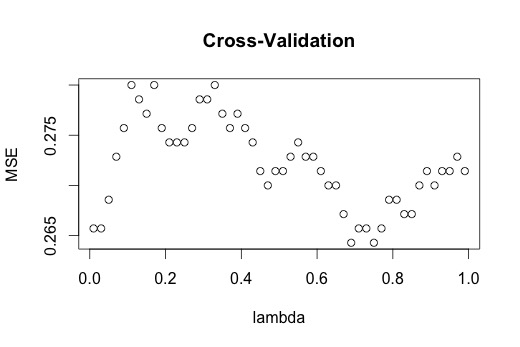
\includegraphics[width=\textwidth, height=4.5cm]{lambda_20}
            \caption{Cross-Validation}\label{lambda_20}
        \end{subfigure}
        \hfil
        \begin{subfigure}[b]{0.475\textwidth}
            \centering
            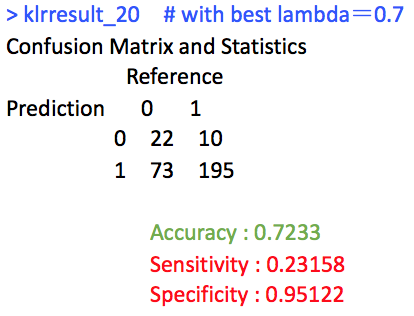
\includegraphics[width=\textwidth, height=4.5cm]{klr_20_best}
            \caption{KLR with best $\lambda=0.7$} \label{klr_20_best}
        \end{subfigure} \\ \hspace{1em}
        \centering
        \begin{subfigure}[b]{0.475\textwidth}
            \centering
            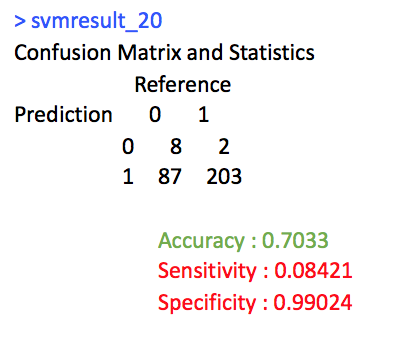
\includegraphics[width=\textwidth, height=4.5cm]{svm_20}
            \caption{\small SVM}\label{svm_20}
        \end{subfigure}
        \hfil
        \begin{subfigure}[b]{0.475\textwidth}
            \centering
            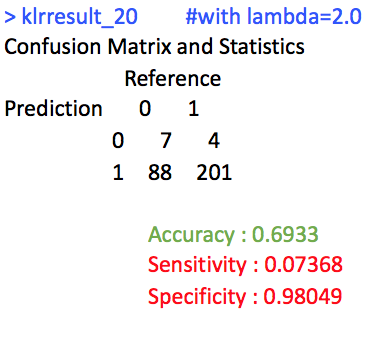
\includegraphics[width=\textwidth, height=4.5cm]{klr_20}
            \caption{\small KLR with $\lambda=2.0$}\label{klr_20}
        \end{subfigure}
        \caption{}
\end{figure}
The results of 20-attribute case is shown in Figure 1. Since the German credit data set is imbalanced which means it has more good credits than bad credits, it is more suitable to look at sensitivity and specificity rather than accuracy. For 20-attribute case, we can get best $\lambda=0.7$ from \reffig{lambda_20}. Kernel Logistic Regression with best $\lambda$ gave better sensitivity than SVM on German Credit data set, and their specificity and accuracy are similar. When we changed $\lambda$ to 2.0, sensitivity decreased but specificity increased. So there is a tradeoff between sensitivity and specificity balanced by $\lambda$.\\

The 15-attribute case and 10-attribute case are respectively shown in Figure 2 and Figure 3. The analyses of 15-attribute case and 10-attribute case are similar to preceding analysis.  Between cases with different number of attributes, as we removed 5 qualitative attributes, there is only slight fluctuation on the performance.

\begin{figure}[!h]
       \centering
        \begin{subfigure}[b]{0.475\textwidth}
            \centering
            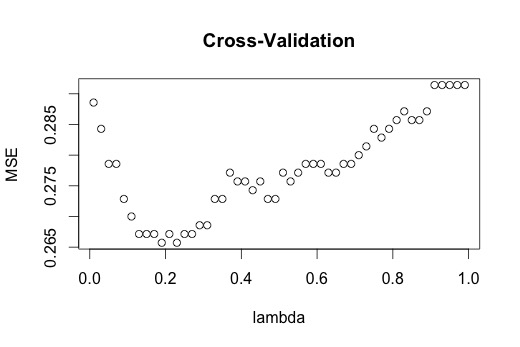
\includegraphics[width=\textwidth, height=4.5cm]{lambda_15.jpeg}
            \caption{\small Cross-Validation}\label{lambda_15.jpeg}
        \end{subfigure}
        \hfil
        \begin{subfigure}[b]{0.475\textwidth}
            \centering
            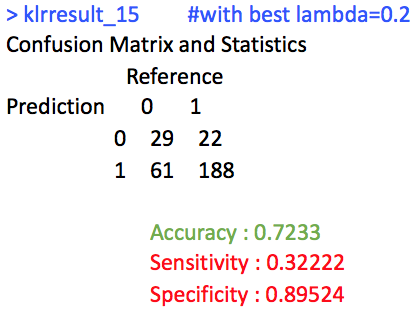
\includegraphics[width=\textwidth, height=4.5cm]{klr_15_best}
            \caption{\small KLR with best $\lambda=0.2$} \label{klr_15_best}
        \end{subfigure} \\ \hspace{1em}
        \centering
        \begin{subfigure}[b]{0.475\textwidth}
            \centering
            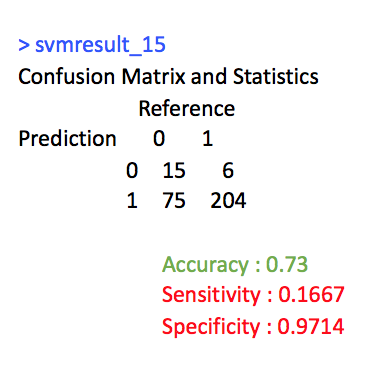
\includegraphics[width=\textwidth, height=4.5cm]{svm_15}
            \caption{\small SVM}\label{svm_15}
        \end{subfigure}
        \hfil
        \begin{subfigure}[b]{0.475\textwidth}
            \centering
            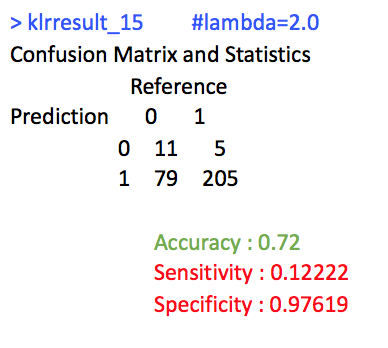
\includegraphics[width=\textwidth, height=4.5cm]{klr_15}
            \caption{\small KLR with $\lambda=2.0$}\label{klr_15}
        \end{subfigure}
        \caption{}
\end{figure}
\begin{figure}[h]
        \centering
        \begin{subfigure}[b]{0.475\textwidth}
            \centering
            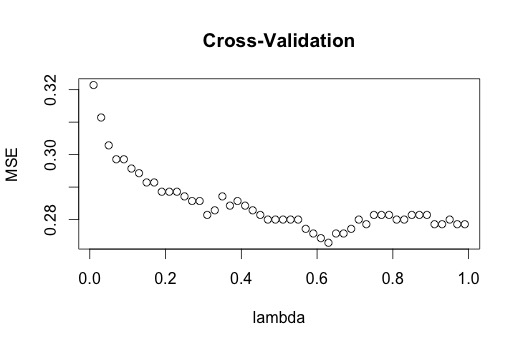
\includegraphics[width=\textwidth, height=4.5cm]{lambda_10}
            \caption{\small Cross-Validation}\label{lambda_10}
        \end{subfigure}
        \hfill
        \begin{subfigure}[b]{0.475\textwidth}
            \centering
            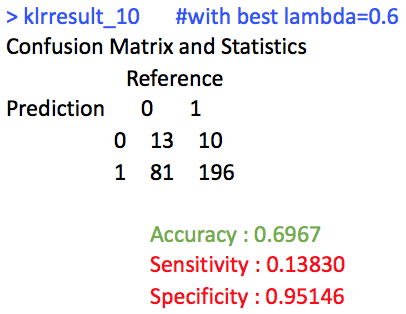
\includegraphics[width=\textwidth, height=4.5cm]{klr_10_best}
            \caption{\small KLR with best $\lambda=0.6$}\label{klr_10_best}
        \end{subfigure} \\ \hfil \hspace{1em}
        \centering
        \begin{subfigure}[b]{0.475\textwidth}
            \centering
            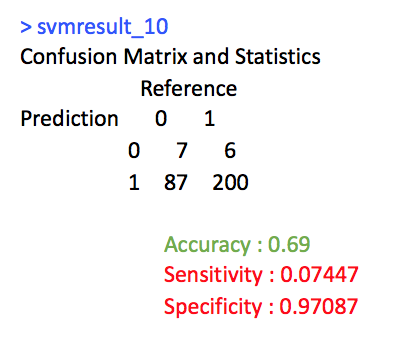
\includegraphics[width=\textwidth, height=4.5cm]{svm_10}
            \caption{\small SVM }\label{svm_10}
        \end{subfigure}
        \hfil
        \begin{subfigure}[b]{0.475\textwidth}
            \centering
            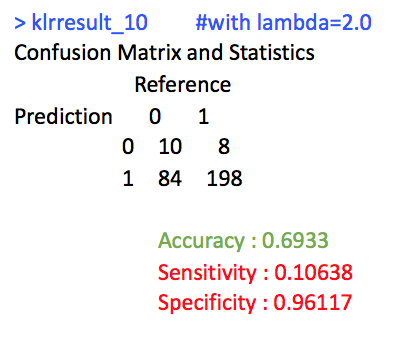
\includegraphics[width=\textwidth, height=4.5cm]{klr_10}
            \caption{\small KLR with $\lambda=2.0$}\label{klr_10}
        \end{subfigure}
       \caption{}
\end{figure}



\subsection{Comments}
~~~~The credit classification performance of Kernel Logistic Regression is comparable with SVM and can be recommended as a method to evaluate credit approval. The advantages of Kernel Logistic Regression compared to SVM is that it provides not only the predicted class, but also the estimated posterior probability of the predicted class which can be used as a confidence measure and sometimes are more useful than the classifications like in credit risk scoring area. And Kernel Logistic Regression can be generalized naturally to M-class classification through kernel multi-logit regression. But Kernel Logistic Regression is computationally more expensive because of the time complexity $O(N^{3})$, and it is hard to specify parameter $c$.

\vspace{6pt}
If the credit data is extremely imbalanced, like the large credit card fraud data set, we should use specific method improvement to deal with this problem. For German Credit data set, we still did not get a good sensitivity in above three cases and original paper$^{[1]}$. We tried considering class weight into SVM on 20-attribute case ($w_0/w_1=N_1/N_0$, $w_i$ is class weight and $N_i$ is the number of class observations), and we got following better result.

\begin{figure}[H]
        \centering
         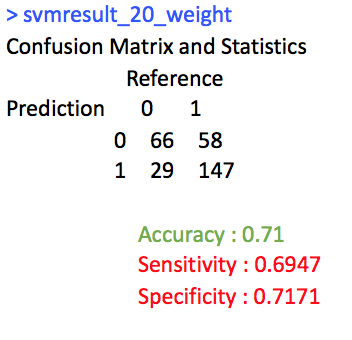
\includegraphics[width=5.5cm,height=5cm]{svm_20_w}
         \caption{\normalsize SVM with class weight }\label{svm_20_w}
\end{figure}

The accuracy is similar to preceding result, but sensitivity is largely improved, and the tradeoff between sensitivity and specificity is more balanced.


\section{Robust Regularized Kernel Regression}
~~~~In Kernel Ridge Regression, squared loss works quite well for observations in which error term is normal distribution and L2 norm constrains coefficients in order to avoid overfitting.  But in practice, we should pay more attention to the data set, because $Y$ may be skewed and cannot be assumed as normal distribution.  In this situation, more frequent outliers will distort prediction because KRR will fit outliers so that the squared loss could decrease significantly.  Thus, we need a loss function which can tolerate more outliers than squared loss.  Besides, we also wish the loss function works better for error with mixture distribution, aggregate distribution and so on.  The following parts will introduce a robust model with Huber loss called RRKR and then compare its performance with KRR.

\subsection{Formula Deduction}
~~~~A Kernel Ridge Regression model is the sum of squared loss and L2 norm, shown as follows:
\begin{equation}
\mathop{argmin}_{\theta \in \mathbb{R}^{p'}} \sum_{i=1}^{n}(Y_i - \phi(X_i)^{\top}\theta)^2 + \lambda\langle\theta,\theta\rangle
\end{equation}
We rewrite the whole function in the following form:
\begin{equation}
\mathop{argmin}_{\theta \in \mathbb{R}^{p'}}\sum_{i=1}^{n} V(Y_i, \phi(X_i)^{\top}\theta)^2 + \lambda\langle\theta,\theta\rangle
\end{equation}
$V(Y_i, \phi(X_i)^{\top}\theta)$ is loss function. Usually we calculate loss with $u_i =  Y_i - \phi(X_i)^{\top}\theta$, so loss function changes to $V(u_i)$. For KRR, $V(u_i) = u_i^2$. \\

In general, outliers are overemphasized using the squared loss in KRR. Although the absolute loss can avoid that problem, it overemphasizes loss on points close to the predicted points. Therefore Huber loss is applied to provide a compound solution, which takes the advantage of both loss functions.  It is defined as follows:
\begin{align}
V(Y_i, \phi(X_i)^{\top}) = V(u_i) =
\begin{cases}
m(2(u_i - \epsilon) - m) & u_i-\epsilon > m \\
u_i^2 & 0 < u_i - \epsilon \leq m\\
0 & |u_i| \leq \epsilon \\
u_i^2 & -m \leq u+\epsilon < 0\\
-m(2(u_i + \epsilon) + m) & u_i + \epsilon < -m \\
\end{cases}
\end{align}
\reffig{huber_loss} shows the difference between squared loss and Huber loss.  Both lines are overlapped when $u$ is small, but Huber loss function doesn't weight too much on large loss.
\begin{figure}[h]
\centering
        \begin{subfigure}[b]{0.475\textwidth}
            \centering
            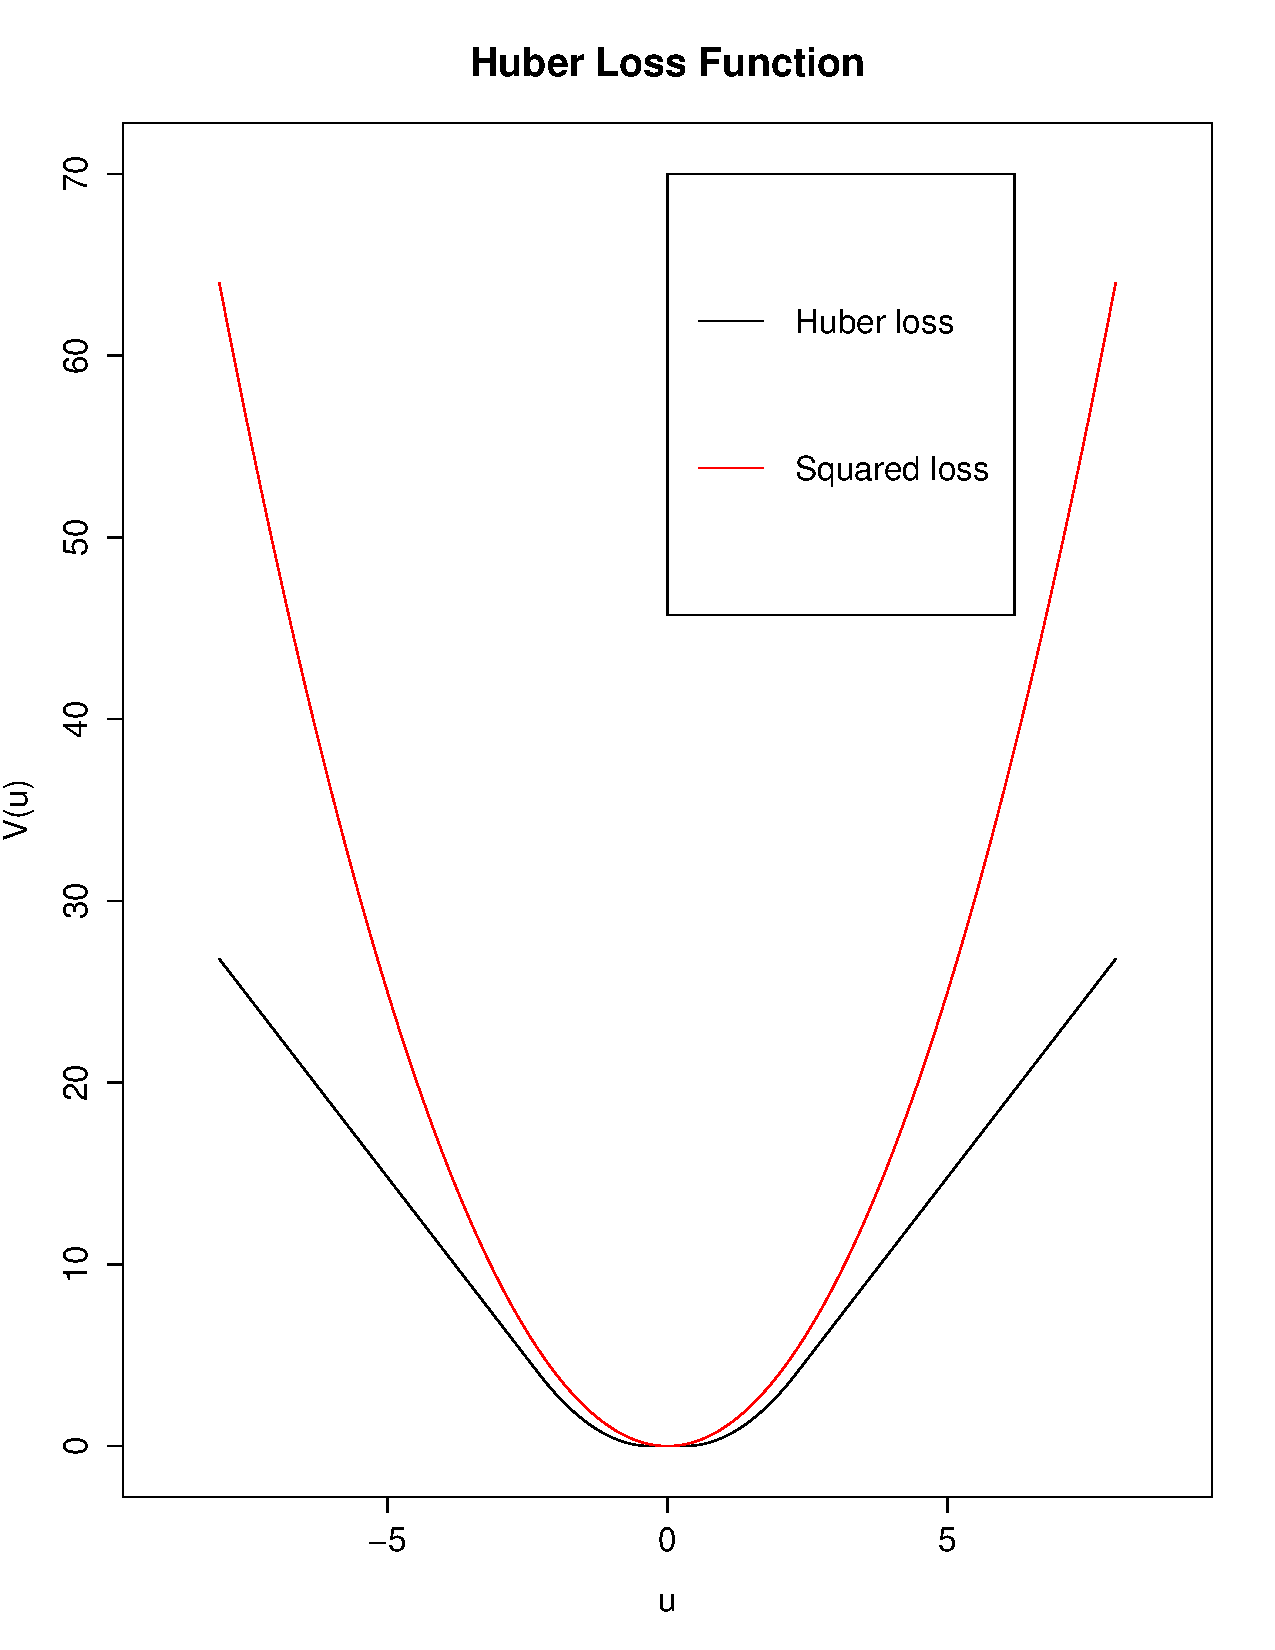
\includegraphics[width=\textwidth, height=4.5cm]{huber_loss.pdf}
            \caption{loss function}\label{huber_loss}
        \end{subfigure}
        \quad
        \begin{subfigure}[b]{0.475\textwidth}
            \centering
            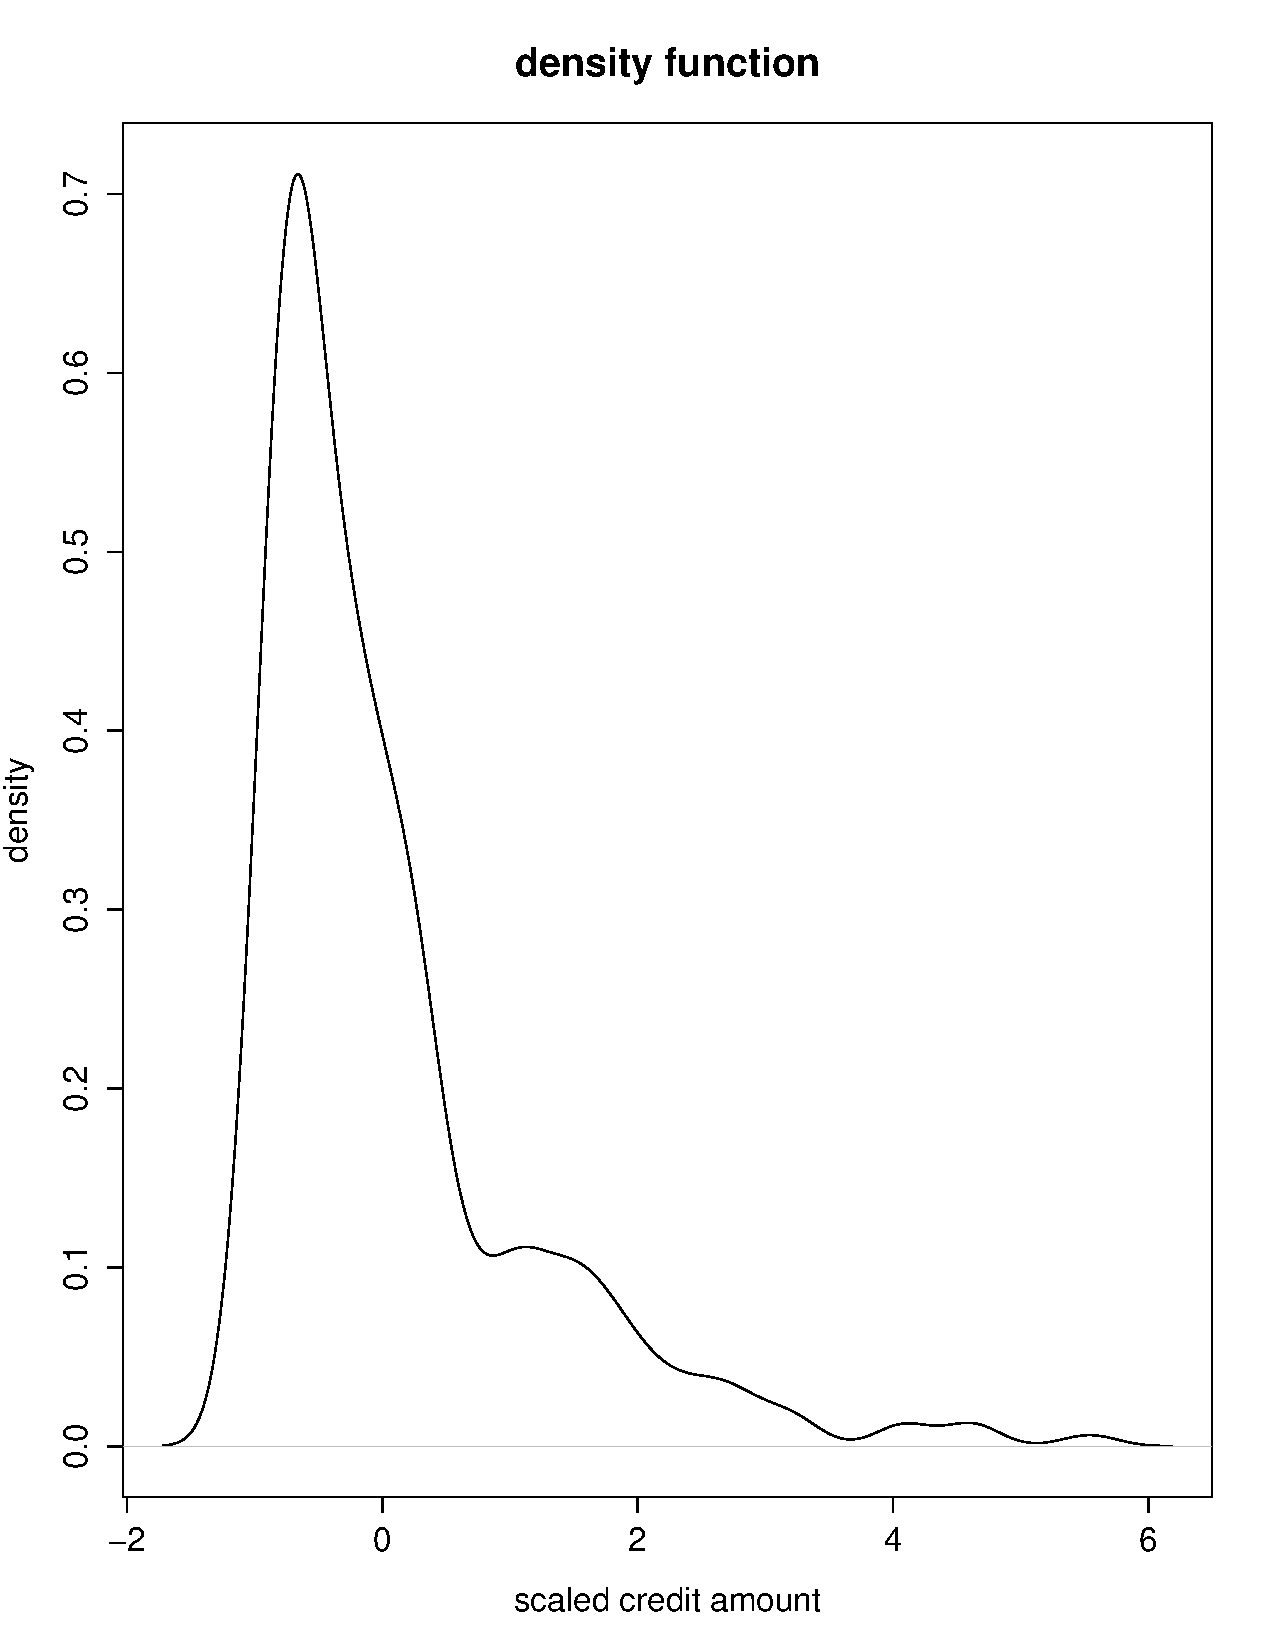
\includegraphics[width=\textwidth, height=4.5cm]{density_15}
            \caption{density function for scaled credit amount}\label{density_15}
        \end{subfigure}
        \caption{}
\end{figure}\\

According to the Representer Theorem$^{[4]}$, there exists an optimum $f(x)$ among the set $\{ f(x) = \phi(X_i)^{\top}\theta | \theta = \sum_i^n  c_i\phi(X_i)\}$ for equation (16) with Huber loss.  In other words, $f(x) = \sum_j^nK(x, x_j)c_j$.  That's what we want and Newton iteration is applied to calculate the numeric result.  First, we substitute $\theta$ with $\sum_i^n  c_i\phi(X_i)$ in equation (16).
\begin{equation}
\begin{split}
E &= \sum_i^n V(y_i - \sum_j^n K(x_i, x_j)c_j) + \lambda \sum_{i,j}^n c_ic_jK(x_i, x_j)\\
 &=  \sum_i^n V(y_i - \sum_j^n K(x_i, x_j)c_j) + \lambda c^\top K c
\end{split}
\end{equation}
We rewrite $V(y - \sum_j^n K(x, x_j)c_j)$.
\begin{align}
V(y - \sum_j^n K(x, x_j)c_j) = V(u) =
\begin{cases}
m(2(u - \epsilon) - m) & S_1 = \{ x|u - \epsilon > m\} \\
(u-\epsilon)^2 & S_2 = \{ x|0 < u-\epsilon \leq m\}\\
0 & S_3 = \{ x | \quad|u| \leq \epsilon\} \\
(u+\epsilon)^2 & S_4 =\{ -m \le u + \epsilon < 0\}\\
-m(2(u + \epsilon) + m) & S_5 =\{ u + \epsilon < -m\}\\
\end{cases}
\end{align}
Then calculate the derivative.
\begin{equation}
\frac{\partial E}{\partial c} = 2(\lambda K c + K I^0Kc + Kq)
\end{equation}
where $q=-I^0y +e$, $I^0$ is a n*n diagonal matrix with diagonal elements, that belong to S2 and S4, being 1 and other elements being 0. $e$ is a vector defined as:
\begin{align}
e_i =
\begin{cases}
m & x_i \in S_1 \\
\epsilon & x_i \in S_2 \\
0 & x_i \in S_3 \\
-\epsilon & x_i \in S_4 \\
-m & x_i \in S_5 \\
\end{cases}
\end{align}
The second order derivative is
\begin{equation}
\frac{\partial^2E}{\partial c c^\top} = 2(\lambda K + K I^0 K )
\end{equation}
~~~~Finally we calculate $c$ by iterations with initial value $c_0$.
\begin{equation}
c^{(t+1)} = c^{(t)} - \left(\frac{\partial^2E}{\partial c c^\top}\right)^{-1}\frac{\partial E}{\partial c} = \left(\lambda K + K I^0 K \right)^{-1}(\lambda K c^{(t)} + K I^0Kc^{(t)} + Kq)
\end{equation}
For each iteration, we partition data into $S_1, \ldots, S_5$ by calculating $u$ through $c^{(t)}$.  Actually, the above $f(x)$ can be solved by the first derivative directly. However, for the following prediction, we actually added an offset to $f(x)$ so that $f(x) =  \phi(X_i)^{\top} + c_0$.  Here Newton method is applied.  For simplicity, we only display the formula without the offset.


\subsection{Results}
~~~~We aimed to predict credit amount given the known data.  In reality, credit amount is calculated by bank but the formula is not simple linear combination, so predicting it with given predictors can test the performance of models.  Here we mainly compared the performance of Kernel Ridge Regression and Robust Regularized Kernel Regression.  \\

We scaled all continuous data so that $(-3.5\sigma, 3.5\sigma)$ should cover most credit amount.  Thus we set $m=3.5$.  we set $\epsilon=0.05$, which means two loss functions are similar with the difference less than 0.05.  \reffig{density_15} shows that the data is skewed so our former assumption may not work.  First we calculated optimum $\lambda$ by cross validation for 15-attribute case.
\begin{figure}[h]
        \centering
        \begin{subfigure}[b]{0.475\textwidth}
            \centering
            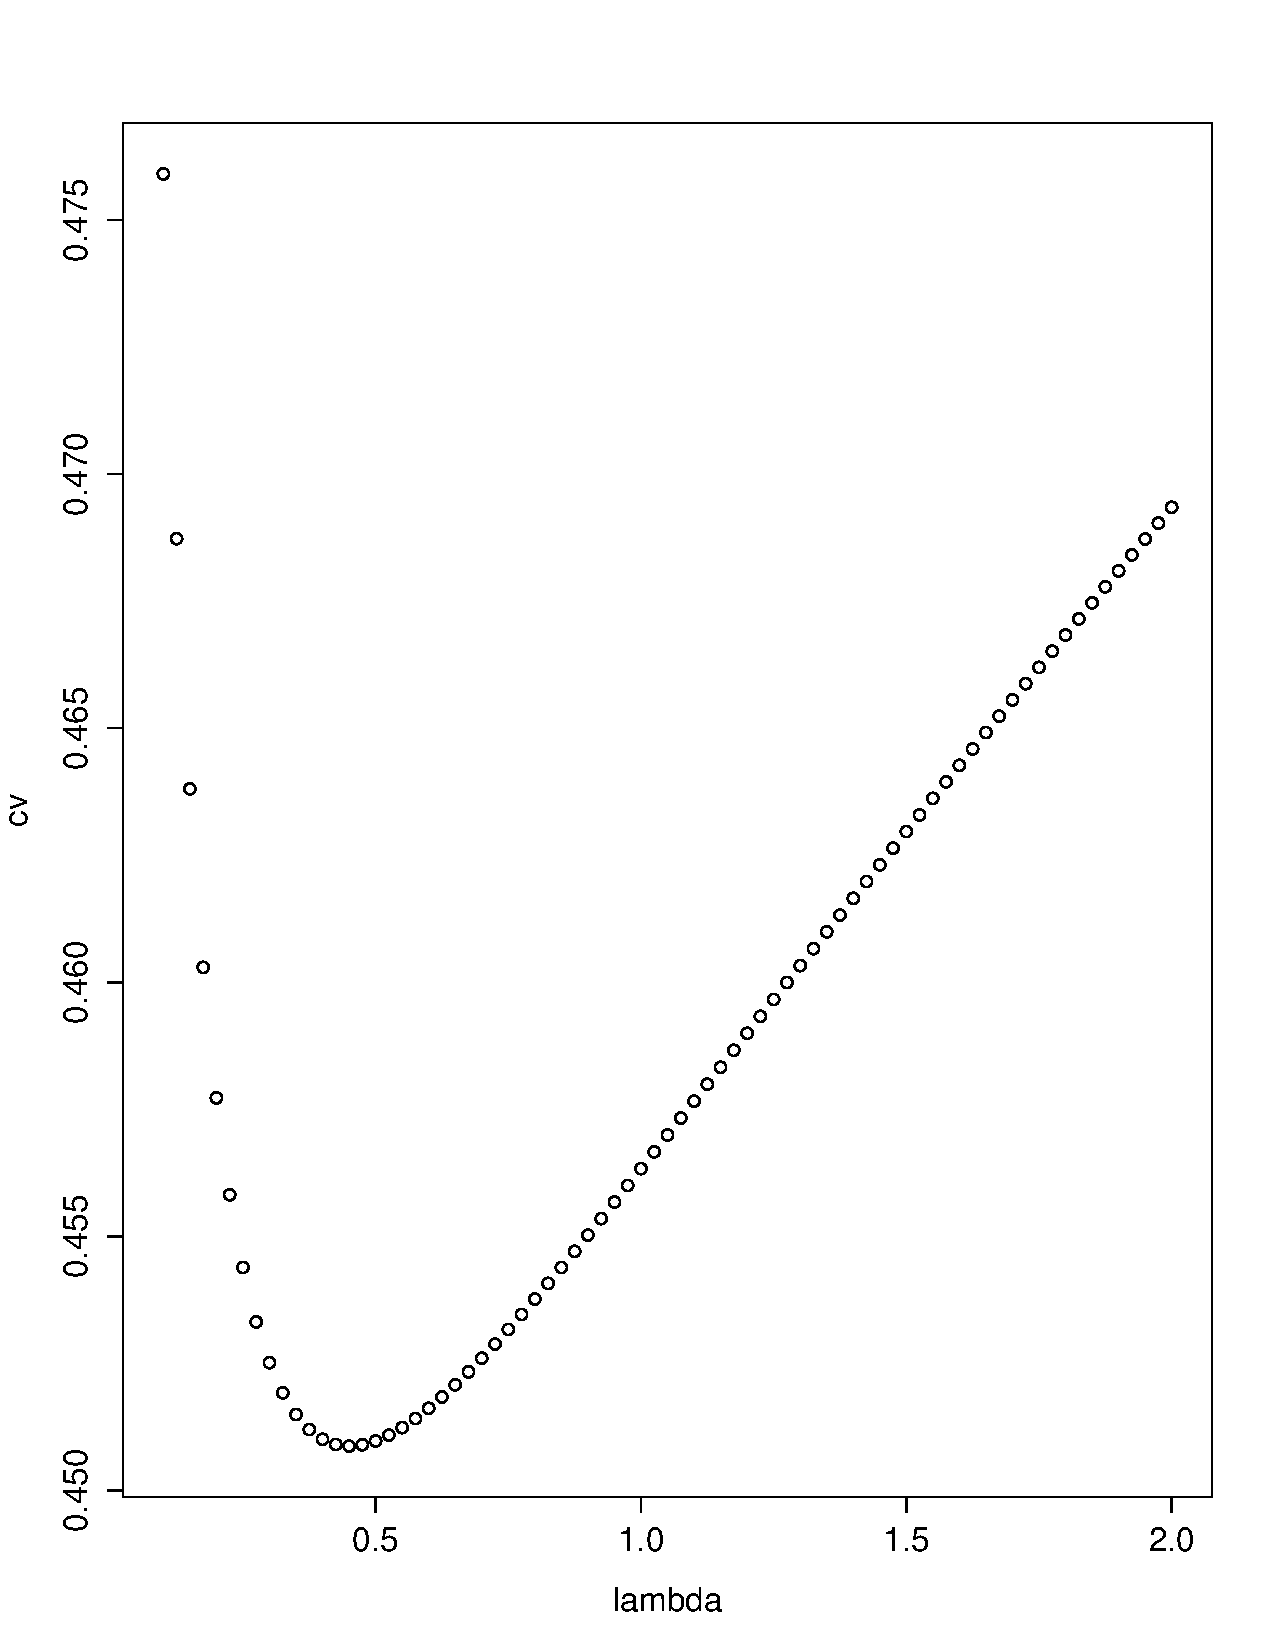
\includegraphics[width=\textwidth, height=4.5cm]{krr_15_cv.pdf}
            \caption{CV for KRR}\label{krr_15_cv}
        \end{subfigure}
        \quad
        \begin{subfigure}[b]{0.475\textwidth}
            \centering
            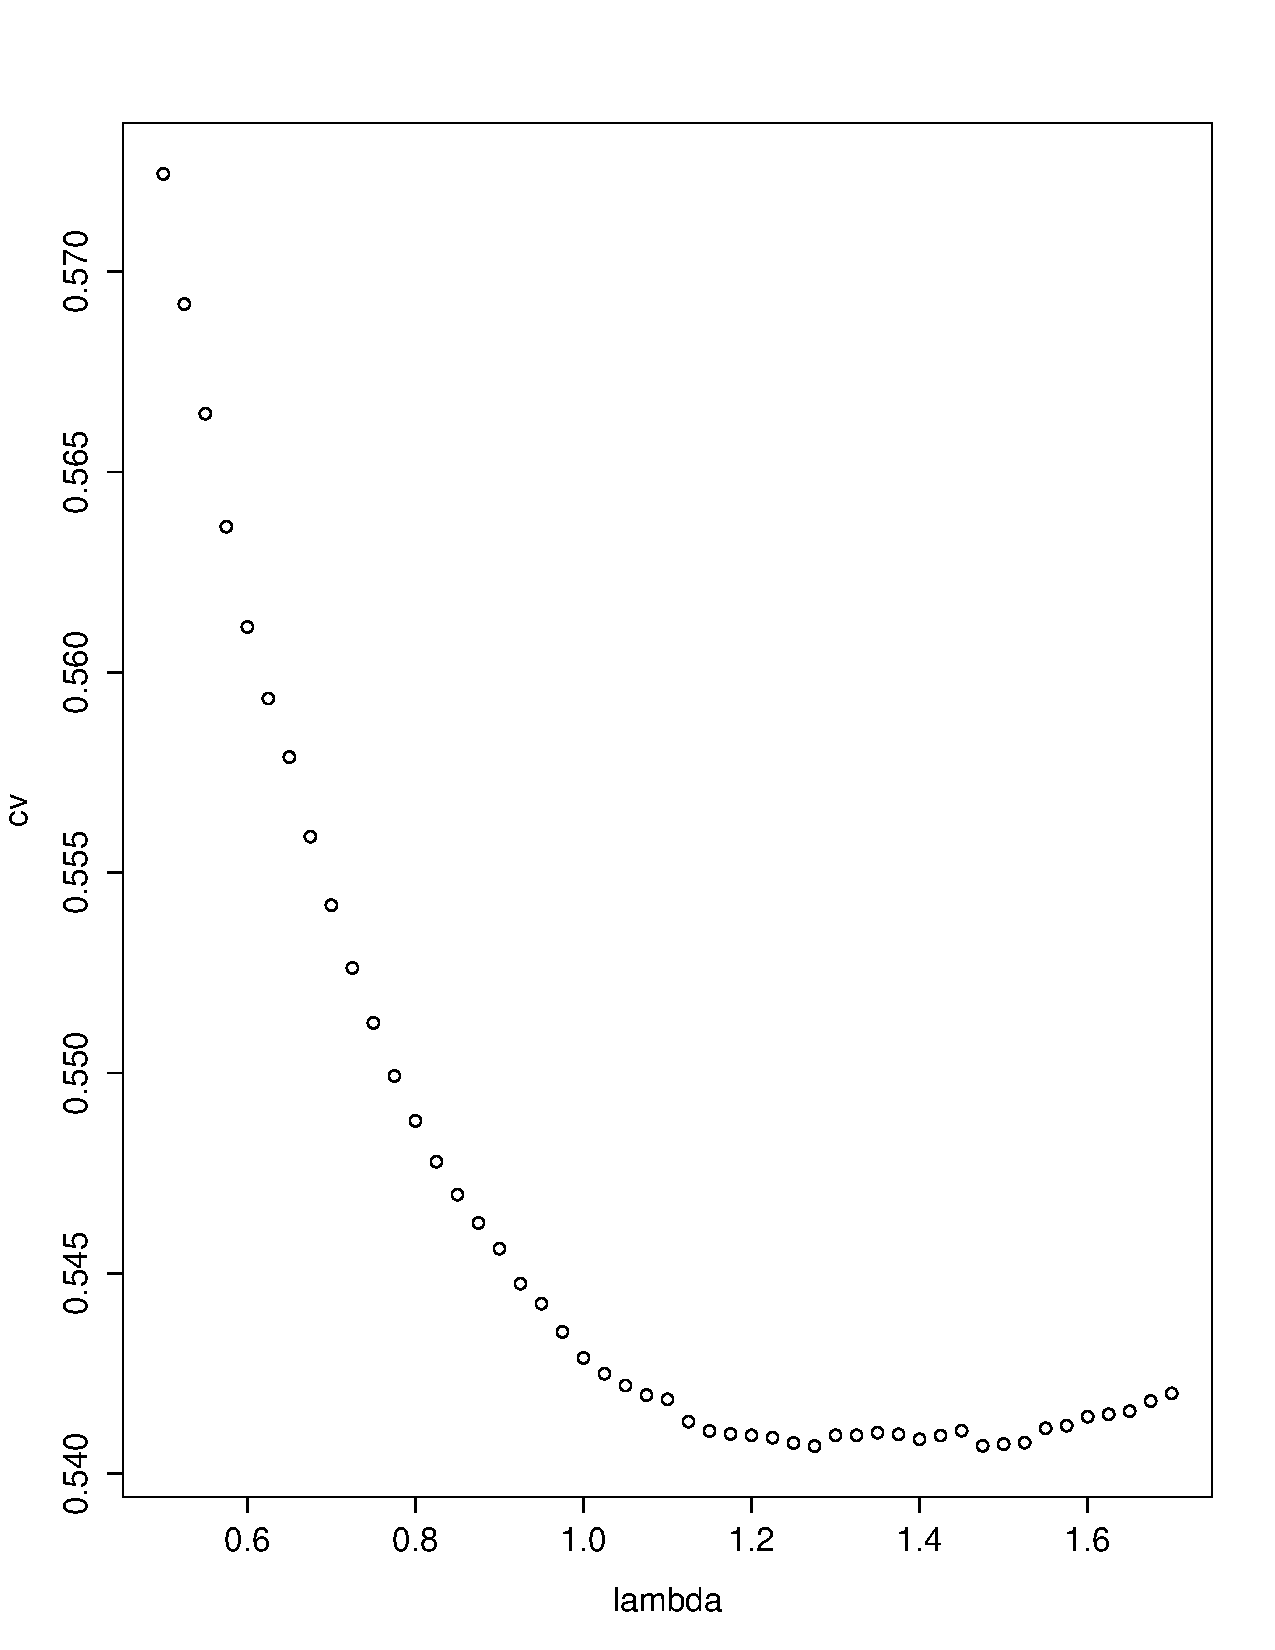
\includegraphics[width=\textwidth, height=4.5cm]{rrkr_15_cv.pdf}
            \caption{CV for RRKR}\label{rrkr_15_cv}
        \end{subfigure}
        \caption{}
\end{figure}
\reffig{krr_15_cv} shows MSE of Kernel Ridge Regression against $\lambda$ while \reffig{rrkr_15_cv} shows MSE of Robust Regularized Kernel Regression.  So we took $\lambda$ as 0.5, 1.2 respectively.  It demonstrates that RRKR puts more weight on penalty for the optimum so that the model could be less overfitting than KRR.\\
\begin{figure}[h]
        \centering
        \begin{subfigure}[b]{0.475\textwidth}
            \centering
            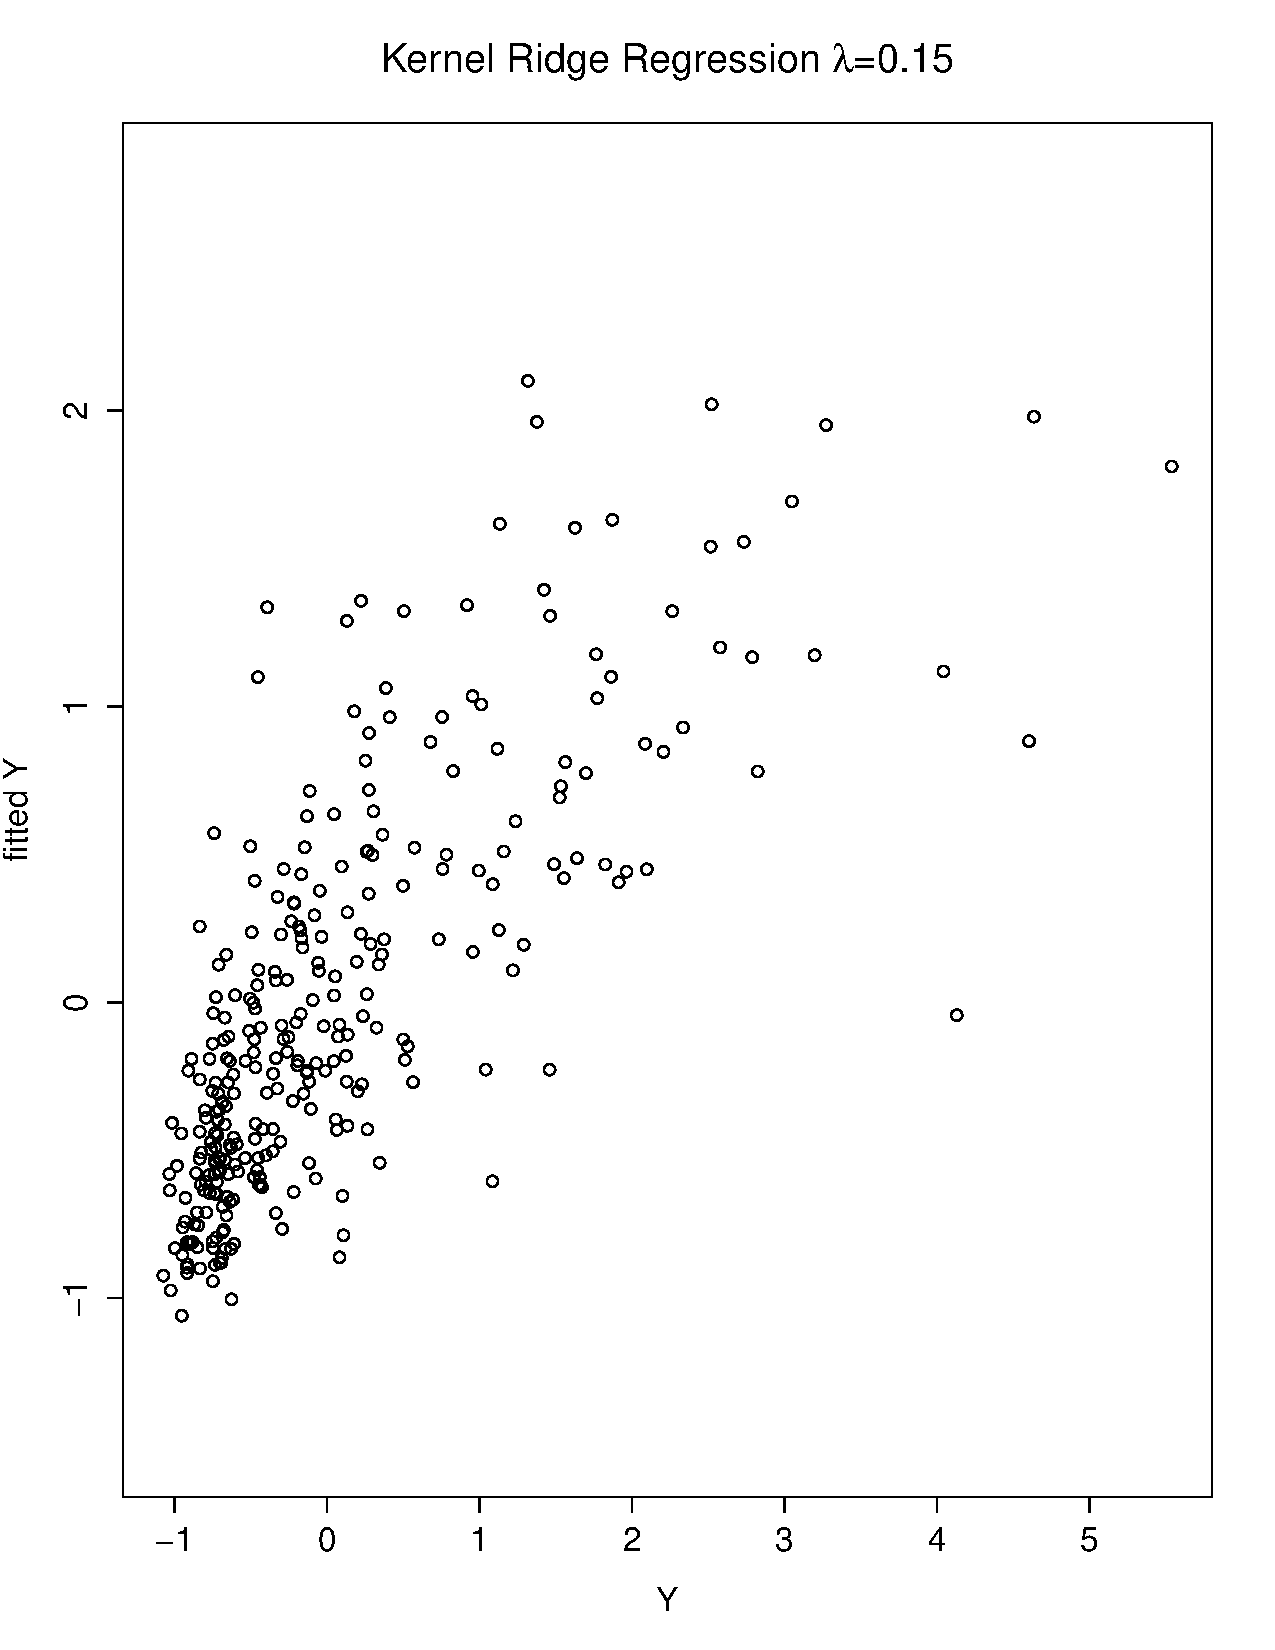
\includegraphics[width=\textwidth, height=4.5cm]{krr_15.pdf}
            \caption{}\label{krr_15}
        \end{subfigure}
        \quad
        \begin{subfigure}[b]{0.475\textwidth}
            \centering
            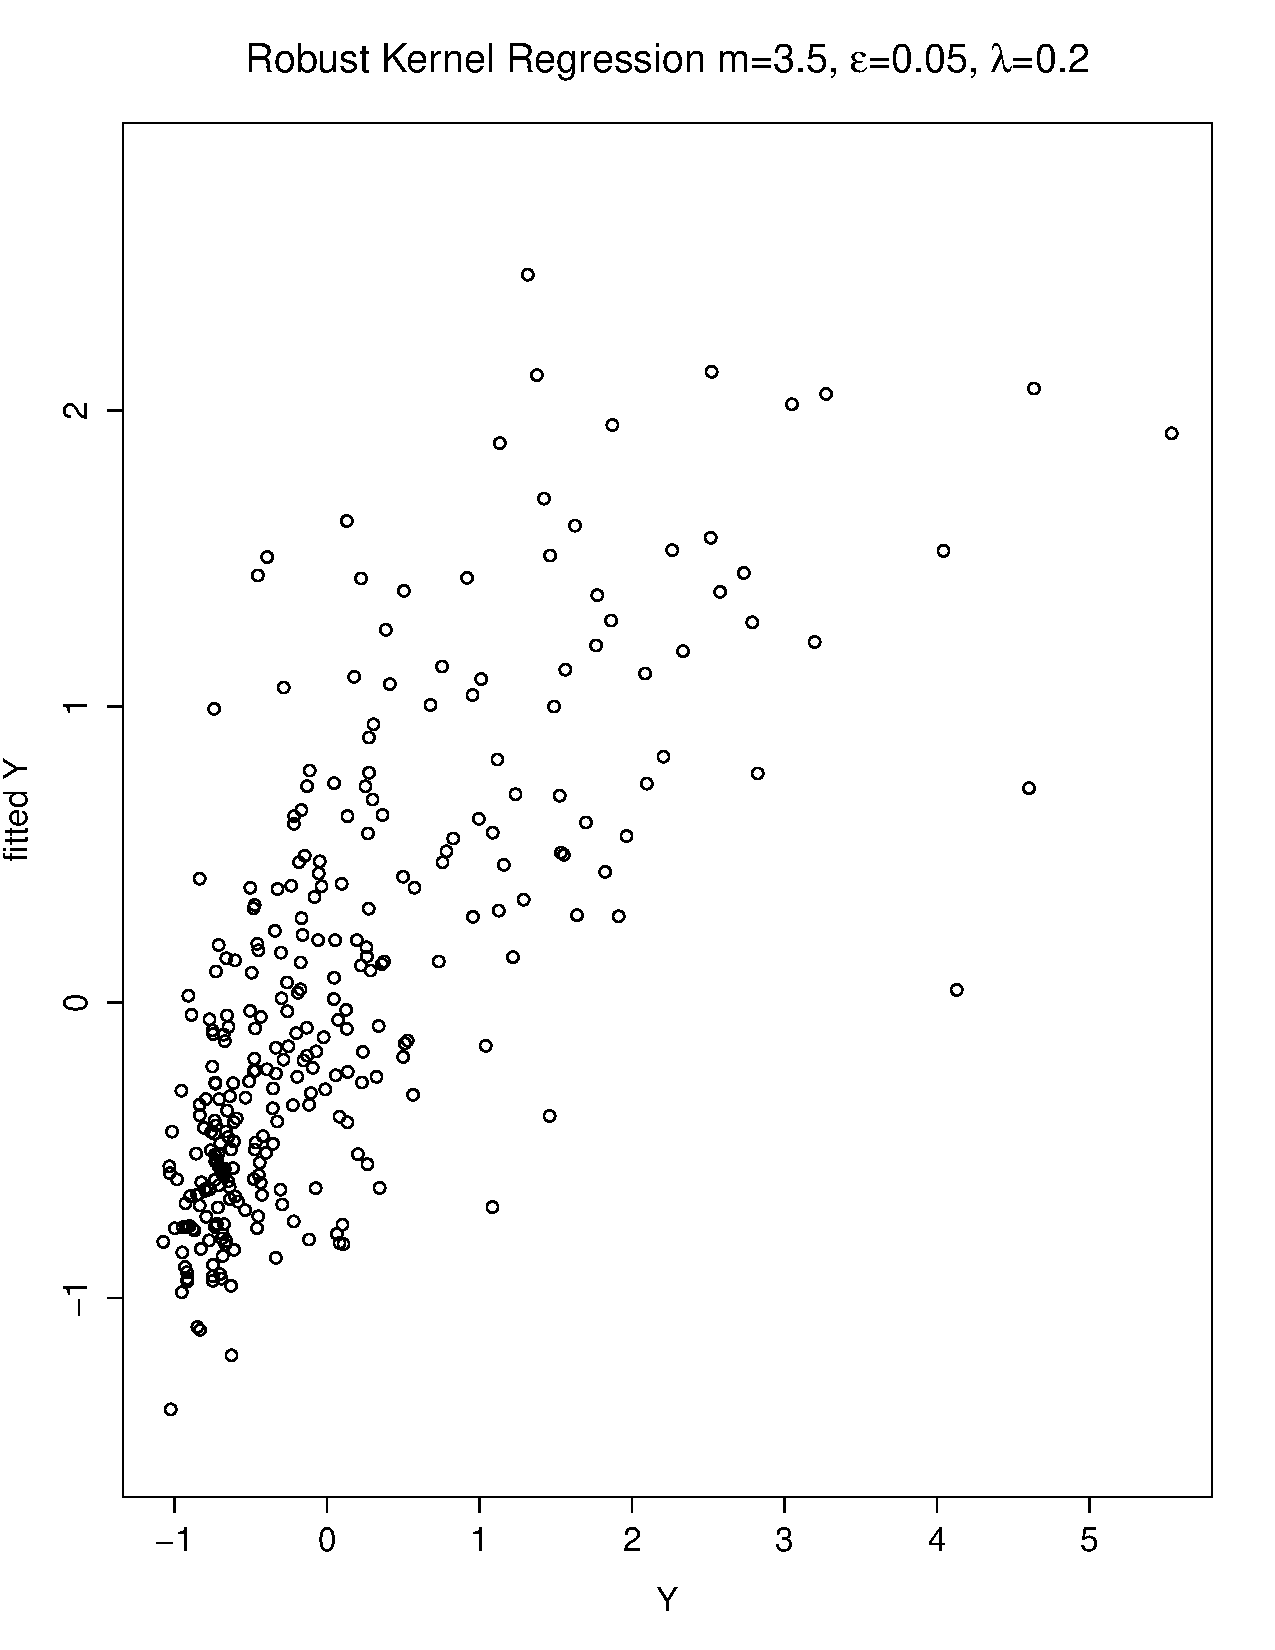
\includegraphics[width=\textwidth, height=4.5cm]{rrkr_15.pdf}
            \caption{}\label{rrkr_15}
        \end{subfigure}
        \caption{}
\end{figure}

\reffig{krr_15} and \reffig{rrkr_15} show predicted credit amounts against real values.  From figures, they seem to have similar performance.  However, if we apply wilcoxon signed rank test$^{[1]}$ to check the distribution of real values with predicted values, p-values are 0.3681 and 0.0651 with respect to KRR and RRKR.  So RRKR performs much better than KRR. \\
\begin{figure}[h]
        \centering
        \begin{subfigure}[b]{0.475\textwidth}
            \centering
            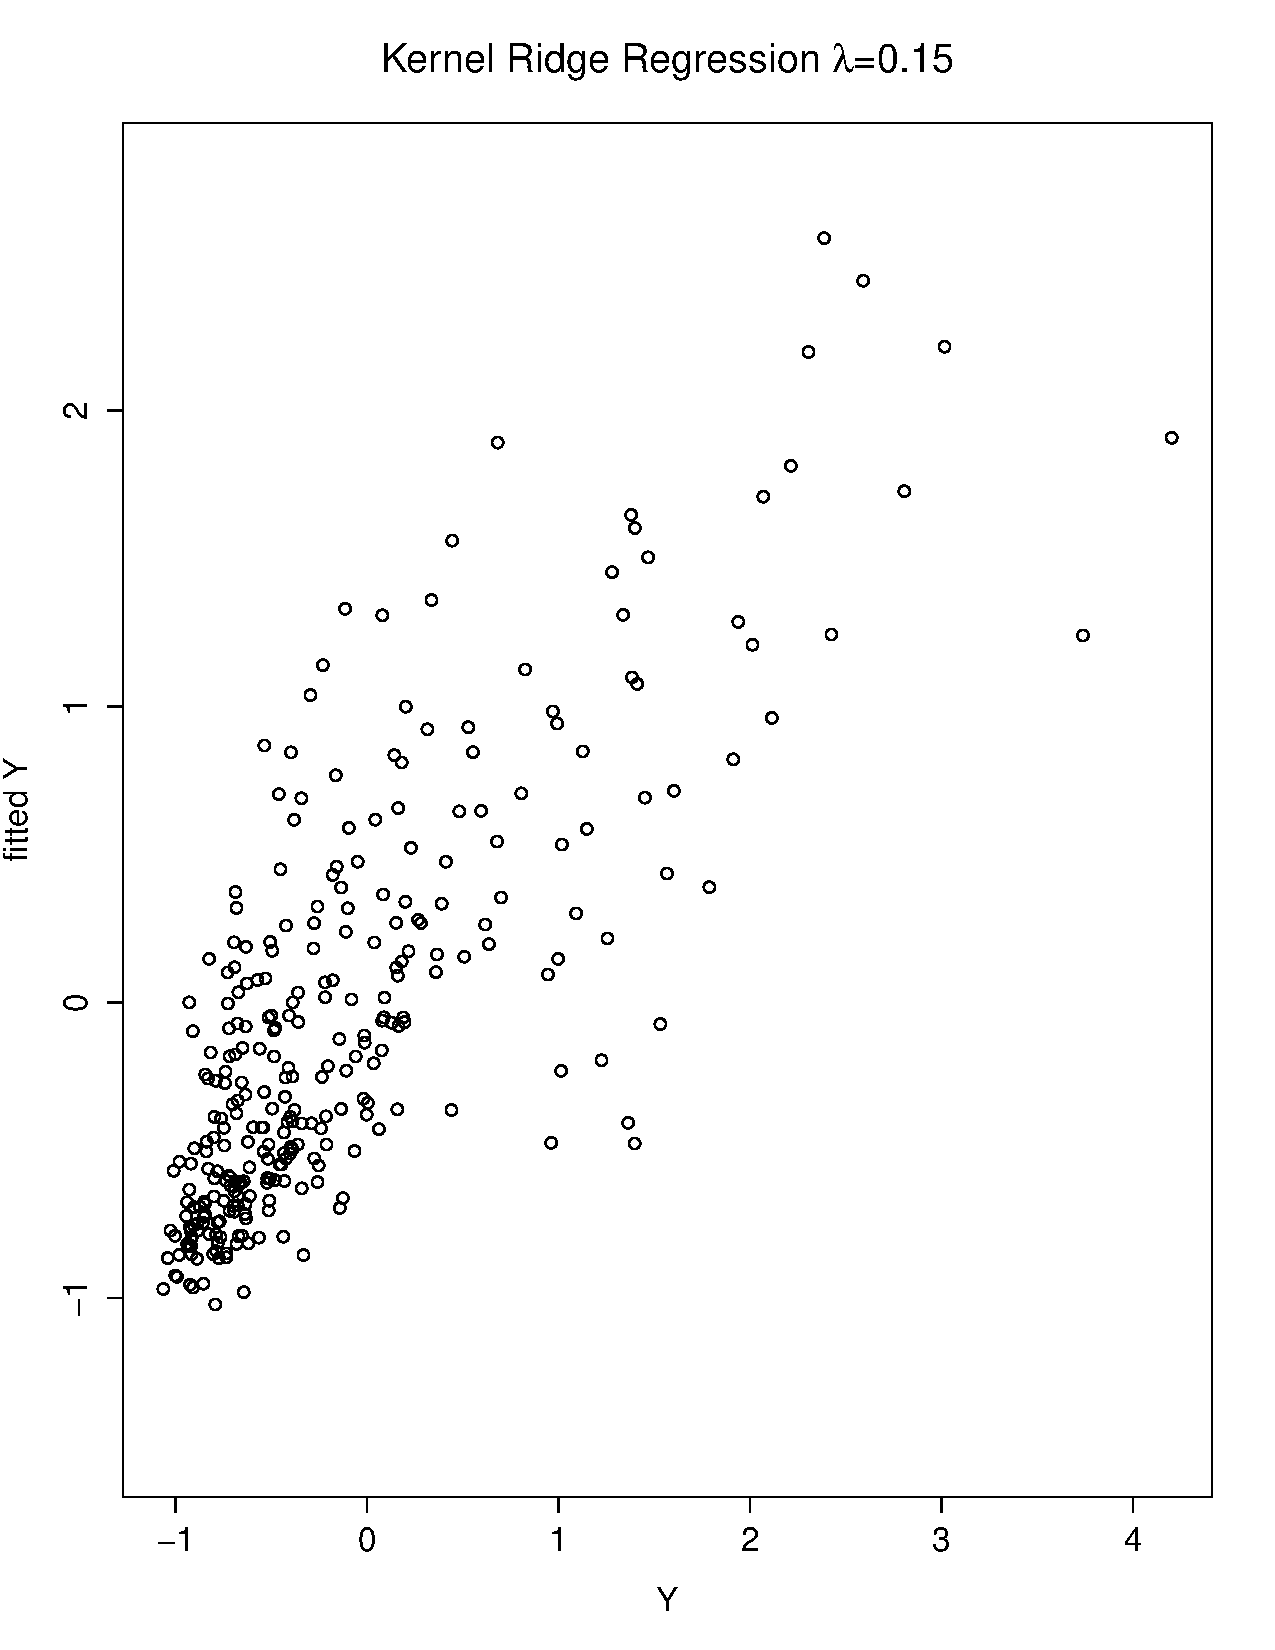
\includegraphics[width=\textwidth, height=4.5cm]{krr_10.pdf}
            \caption{}\label{krr_10}
        \end{subfigure}
        \quad
        \begin{subfigure}[b]{0.475\textwidth}
            \centering
            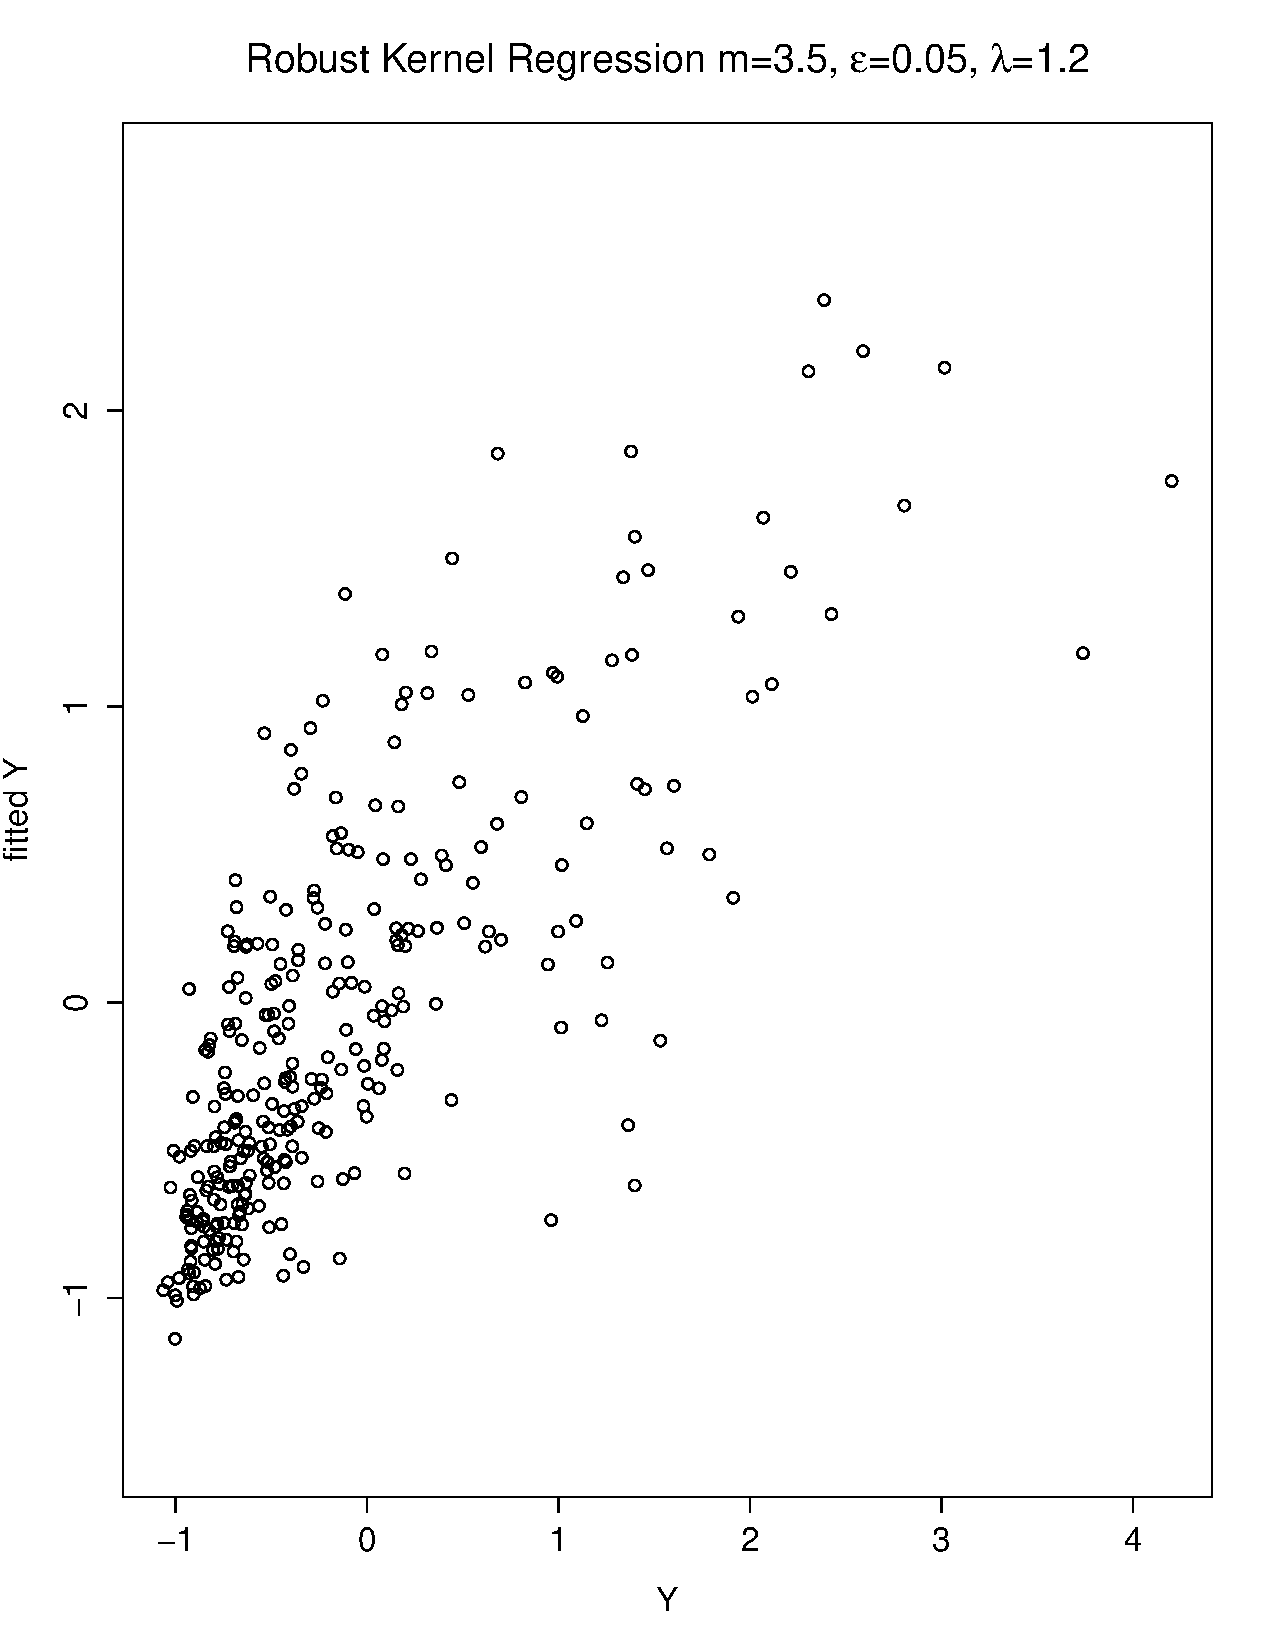
\includegraphics[width=\textwidth, height=4.5cm]{rrkr_10.pdf}
            \caption{}\label{rrkr_10}
        \end{subfigure}
        \caption{}
\end{figure}

We also tested KRR and RRKR on the 10-attribute case.  The result is similar.  $\lambda$s are still 0.5 and 1.2.  However, for the prediction, both method improve a lot. \reffig{krr_10} and \reffig{rrkr_10} show the scatter plots.  For wilcoxon signed rank test, p-values of KRR and RRKR are 0.0005584 and 0.0001922 respectively. It suggests that KRR and RRKR have similar performance, given a proper number of variables.  But in reality, it's hard to decide a proper number of variables so it is robust to apply RRKR.  It performs at least as well as KRR does and prediction is not largely changed by larger number of variables.

\subsection{Comments}
~~~~In the last subsection, we see the advantage of Robust Regularized Kernel Regression.  Here we discuss some problems when applying it.  The first is time-consuming.  When data grows, although its time complexity is polynomial, it takes much more time than KRR.  Choosing $m$ and $\epsilon$ is another problem.  Maybe we can use cross validation.  But in that case, we have three variables including $\lambda$ so computation is large.  A proper initial value is necessary, otherwise the final result may not converge.  It is hard to guess the set of proper initial values when it is small. But overall RRKR is a good choice with high accuracy.

\section{Conclusions}
~~~~In this paper, we compared Support Vector Machine with Kernel Logistic Regression for discrete output like credit risk classification and compared Kernel Ridge Regression with Robust Regularized Kernel Regression for continuous output like credit amount prediction. For discrete case, we show that SVM and KLR have similar performance. For continuous case, we show that the performance of RRKR is at least as good as the performance of KRR.  When data is skewed, RRKR can still work well. The preceding sections include general theory frameworks, results and comments we concluded in practical problems.

\vspace{8pt}
\textbf{\Large{\center{Reference}}}

\vspace{8pt}
\noindent[1] S. P. Rahayu, S. W. Purnami, A. Embong, \lq\lq Applying Kernel Logistic Regression in Data Mining to Classify Credit Risk\rq\rq, Information Technology, 2008. ITSim 2008. International Symposium on  (Volume:2), 26-28 Aug. 2008.

\vspace{6pt}
\noindent[2] Jianke Zhu, Steven C. H. Hoi, Michael Rung-Tsong Lyu, \lq\lq Robust Regularized Kernel Regression\rq\rq, IEEE transactions on systems, man, and cybernetics. Part B, Cybernetics: a publication of the IEEE Systems, Man, and Cybernetics Society (Impact Factor: 6.22), Dec. 2008.

\vspace{6pt}
\noindent[3] UCI Repository of Machine Learning Databases: http://archive.ics.uci.edu/ml/

\vspace{6pt}
\noindent[4] Bernhard Scholkopf, Ralf Herbrich, Alex J. Smola, \lq\lq A Generalized Representer Theorem\rq\rq, Computational Learning Theory, Springer Berlin Heidelberg, 2001, pp. 416-426.

\vspace{6pt}
\noindent[5] Wilcoxon, Frank. \lq\lq Individual comparisons by ranking methods.\rq\rq Biometrics bulletin 1.6 (1945): 80-83.
\end{document}
